% This is "sig-alternate.tex" V2.1 April 2013
% This file should be compiled with V2.5 of "sig-alternate.cls" May 2012
%
% This example file demonstrates the use of the 'sig-alternate.cls'
% V2.5 LaTeX2e document class file. It is for those submitting
% articles to ACM Conference Proceedings WHO DO NOT WISH TO
% STRICTLY ADHERE TO THE SIGS (PUBS-BOARD-ENDORSED) STYLE.
% The 'sig-alternate.cls' file will produce a similar-looking,
% albeit, 'tighter' paper resulting in, invariably, fewer pages.
%
% ----------------------------------------------------------------------------------------------------------------
% This .tex file (and associated .cls V2.5) produces:
%       1) The Permission Statement
%       2) The Conference (location) Info information
%       3) The Copyright Line with ACM data
%       4) NO page numbers
%
% as against the acm_proc_article-sp.cls file which
% DOES NOT produce 1) thru' 3) above.
%
% Using 'sig-alternate.cls' you have control, however, from within
% the source .tex file, over both the CopyrightYear
% (defaulted to 200X) and the ACM Copyright Data
% (defaulted to X-XXXXX-XX-X/XX/XX).
% e.g.
% \CopyrightYear{2007} will cause 2007 to appear in the copyright line.
% \crdata{0-12345-67-8/90/12} will cause 0-12345-67-8/90/12 to appear in the copyright line.
%
% ---------------------------------------------------------------------------------------------------------------
% This .tex source is an example which *does* use
% the .bib file (from which the .bbl file % is produced).
% REMEMBER HOWEVER: After having produced the .bbl file,
% and prior to final submission, you *NEED* to 'insert'
% your .bbl file into your source .tex file so as to provide
% ONE 'self-contained' source file.
%
% ================= IF YOU HAVE QUESTIONS =======================
% Questions regarding the SIGS styles, SIGS policies and
% procedures, Conferences etc. should be sent to
% Adrienne Griscti (griscti@acm.org)
%
% Technical questions _only_ to
% Gerald Murray (murray@hq.acm.org)
% ===============================================================
%
% For tracking purposes - this is V2.0 - May 2012

\documentclass{sig-alternate-05-2015}

\usepackage[gen]{eurosym}
\usepackage{hyperref} % for autoref
\usepackage{graphicx}

\pagenumbering{arabic}
\graphicspath{{./figures/}}

\begin{document}

% Copyright
\setcopyright{acmcopyright}
%\setcopyright{acmlicensed}
%\setcopyright{rightsretained}
%\setcopyright{usgov}
%\setcopyright{usgovmixed}
%\setcopyright{cagov}
%\setcopyright{cagovmixed}


% DOI
\doi{10.475/123_4}

% ISBN
\isbn{123-4567-24-567/08/06}

%Conference
%\conferenceinfo{PLDI '13}{June 16--19, 2013, Seattle, WA, USA}

%\acmPrice{\$15.00}

%
% --- Author Metadata here ---
%\conferenceinfo{WOODSTOCK}{'97 El Paso, Texas USA}
%\CopyrightYear{2007} % Allows default copyright year (20XX) to be over-ridden - IF NEED BE.
%\crdata{0-12345-67-8/90/01}  % Allows default copyright data (0-89791-88-6/97/05) to be over-ridden - IF NEED BE.
% --- End of Author Metadata ---

\title{The Sybil Attack - Theory and Practice}
% \subtitle{[Extended Abstract]
% \titlenote{A full version of this paper is available as
% \textit{Author's Guide to Preparing ACM SIG Proceedings Using
% \LaTeX$2_\epsilon$\ and BibTeX} at
% \texttt{www.acm.org/eaddress.htm}}}
%
% You need the command \numberofauthors to handle the 'placement
% and alignment' of the authors beneath the title.
%
% For aesthetic reasons, we recommend 'three authors at a time'
% i.e. three 'name/affiliation blocks' be placed beneath the title.
%
% NOTE: You are NOT restricted in how many 'rows' of
% "name/affiliations" may appear. We just ask that you restrict
% the number of 'columns' to three.
%
% Because of the available 'opening page real-estate'
% we ask you to refrain from putting more than six authors
% (two rows with three columns) beneath the article title.
% More than six makes the first-page appear very cluttered indeed.
%
% Use the \alignauthor commands to handle the names
% and affiliations for an 'aesthetic maximum' of six authors.
% Add names, affiliations, addresses for
% the seventh etc. author(s) as the argument for the
% \additionalauthors command.
% These 'additional authors' will be output/set for you
% without further effort on your part as the last section in
% the body of your article BEFORE References or any Appendices.

\numberofauthors{1} %  in this sample file, there are a *total*
% of EIGHT authors. SIX appear on the 'first-page' (for formatting
% reasons) and the remaining two appear in the \additionalauthors section.
%
\author{
% You can go ahead and credit any number of authors here,
% e.g. one 'row of three' or two rows (consisting of one row of three
% and a second row of one, two or three).
%
% The command \alignauthor (no curly braces needed) should
% precede each author name, affiliation/snail-mail address and
% e-mail address. Additionally, tag each line of
% affiliation/address with \affaddr, and tag the
% e-mail address with \email.
%
% 1st. author
\alignauthor
Kelong Cong\\
       \affaddr{Delft University of Technology}\\
       \email{k.cong@student.tudelft.nl}
}

\maketitle
\begin{abstract}
  TODO
\end{abstract}

\section{Introduction}
Electronic commerce and online social networks are common phenomenons at the
present time. They allow us to orchestrate many aspects of our lives in the
comfort of our homes, behind the monitors of our devices. An online identity is
often required to use such services, for examples we must create an account to
Tweet\footnote{A message sent using Twitter is a Tweet.} our friend, who must
also have an account. In this scenario, users can choose to remain psudonymous
if they are careful, where their real-life identity is uncorrelated with their
online identity. % privacy

While creating pseudonyms is useful for protecting users' privacy, it also opens
an alleyway for attackers. The Sybil attack, first described by
Douceur\cite{douceur2002sybil}, is an attack where an entity can assume multiple
identities or Sybils, and then attack either another entity or undermine the
whole system. For example, a malicious Twitter user can create many fake
identities and have the fake identities follow his real identity, thus creating
a false reputation. It is one of the most important attacks because it leads to
a large number of consequences including but not limited to spreading false
information, identity theift\cite{bilge2009all} and ballot
stuffing\cite{bhattacharjee2005avoiding}. Furthermore, to the best of our
knowledge, there is no general solution for preventing the Sybil attack.

In this work, we survey various aspects of the Sybil attack. But in contrast
with previous surveys, we include both the theoretical and practical aspects.
First, we describe the Sybil attack in more detail and and illustrate its
importance by looking at how researchers and black-hat hackers mounted the
attack on real-world e-commerce and online social network systems in
\autoref{sec:sybil}. Since there is a large variety of Sybil attack defence
mechanisms, from using trusted-third-party to exploiting the graph
characteristics in online social networks, thus we classify these mechanisms by
their ``main idea'' in \autoref{sec:defences}. Finally we present the related
work and conclude in \autoref{sec:related} and \autoref{sec:summary}.

%%% Local Variables:
%%% mode: latex
%%% TeX-master: "main"
%%% End:


\section{Motivation}\label{sec:motivation}
We begin our survey by showing some alarming Sybil attacks happening in the
real-world. Social network and micro-blogging websites are popular platforms for
organisations to improve public relations and their reputation, but they are
also platforms to spread propoganda. A recent article in the Atlantic described
how Twitter bots (Sybils) are shaping the 2016 US presidential
election\cite{atlantictwitterbots}. Over a third of pro-Trump tweets and almost
a fifth of pro-Clinton tweets, totalling at about 1 million, came from bots. The
article questions whether the bots are a threat to democracy because opinions of
real users are eclipsed by spam of bots.

\begin{figure}
  \centering
  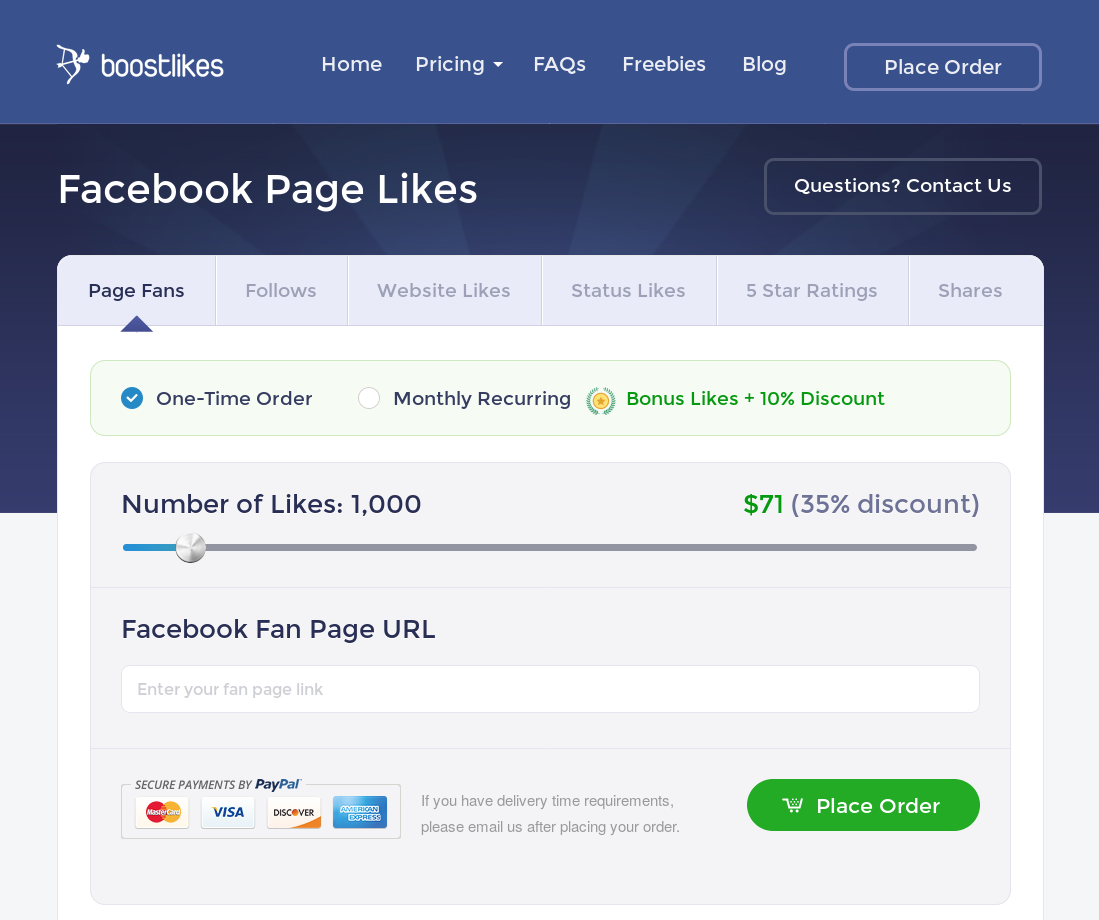
\includegraphics[width=\linewidth]{boostlikes}
  \caption{Screenshot of the Facebook likes service page of boostlikes.com.}
  \label{fig:boostlikes}
\end{figure}

\begin{figure*}
  \centering
  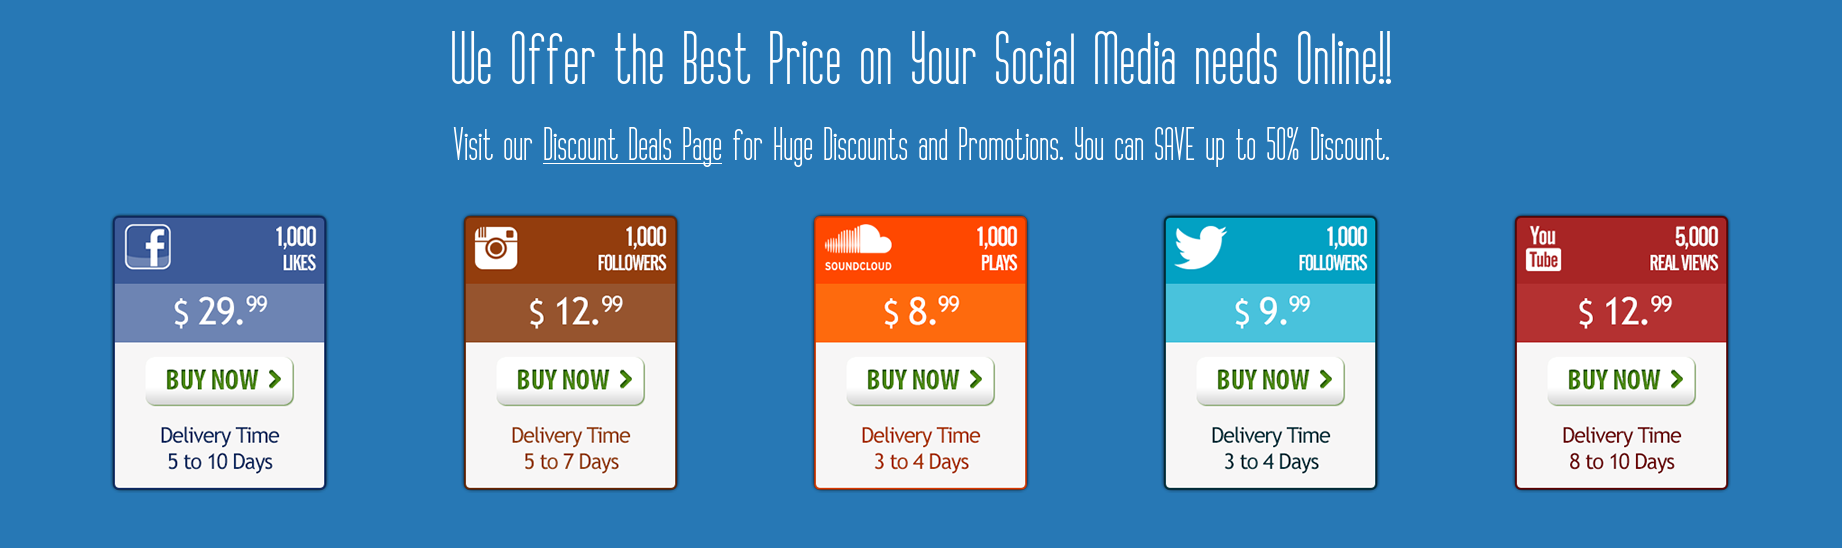
\includegraphics[width=\textwidth]{socialformulae}
  \caption{Screenshot of the main banner on socialformulae.com.}
  \label{fig:socialformulae}
\end{figure*}

Using Sybils to manipulate public opinion is not only accessible to campaigners
with a large budget. There are marketplaces where anybody can purchase
reputation scores such as Twitter followers. BoostLikes shown on
\autoref{fig:boostlikes} is a professionally presented website, it offers a
large range of services including Facebook likes, Twitter followers, Instagram
followers and YouTube views\footnote{Facebook is possibly the largest social
  network website at the time of writing. Instagram is a social network website
  designed for sharing photos. YouTube is a video sharing website.}.
SocialFormulae (\autoref{fig:socialformulae}) is a similar service but at a much
lower price point, one thousand Twitter followers is only \$9.99. There can be
little doubt that those companies use automated bots to provide their services.
% one thousand likes cost \$71 at the time of writing. 

SadBotTrue and its related website Socialpuncher publishes studies on social
media fraud. Two of their studies is particularly useful for demonstrating the
scale of the Sybil attack on Twitter. Firstly, there exist a botnet that consist
of 3 million accounts. Since their creation, they generated 2.6 billion tweets.
Surprisingly, all of the 3 million accounts were created on the same day and the
account names are simply numbered sequentially\cite{sadbottrue}. Such an obvious
activity should be easily detectable by Twitter, but these accounts are still
not closed at the time of writing. Secondly, the top-100 Twitter users have 523
million unique followers between them, but 310 million are bots, that is almost
60\%\cite{socialpuncher}. Suppose the bots all belong to the same attacker, then
they can effectively suppress the opinions of the real users.

Clearly, the defence mechanisms employed by social network and micro-blogging
websites are not adaquate to combat the Sybil attack. If the Sybils infiltrate
even more of our cyberspace, then it may become a form of censorship.
Effectively taking away our right to freedom of speech.

Speaking of censorship, many users use Tor (The Onion
Router)~\cite{dingledine2004tor} to access the uncensored internet when living
in authoritarian regimes such as China, or intelligence agencies from doing
illegal mass surveillence. Unfortunately, Tor suffered a Sybil attack. In
January 2014, 115 relays joined the Tor network. Six months later, it was
discovered that those relays were using a protocol vulnerability to deanonymise
users and find the location of hidden services. It is unclear to the Tor
developers which users are affected or what information was retrieved, thus it
is assumed that users who used Tor between that period are all
affected\cite{torsybil}. In fact, Tor depends on the fact that majority of the
relays are good to guarantee anonymity with a high probability. If the network
is infiltrated by a large number of Sybils then users can be easily
deanonymised.

These example demonstrate a big problem with in the popular social network
websites and anonymous communication tool we use today. A lot of Sybils
controlled by an attacker can censor content and track user behaviour. In the
next section, we zoom in on the practical attacks and grouped them by the
underlying application.

%%% Local Variables:
%%% mode: latex
%%% TeX-master: "main"
%%% End:


\section{The Sybil Attack}\label{sec:sybil}
The sybil attack is coined by Douceur\cite{douceur2002sybil} in 2002 in the
context of P2P (peer-to-peer) systems. But people were well aware of it before
2002. For instance in 2001, Friedman and Resnick used the term ``cheap
pseudonyms'' to describe sybils~\cite{resnick2001social}. In this section, we
introduce the key theoretical results and the definitions used in the remainder
of this survey.

\subsection{Theoretical Results}\label{sec:sybil-theory}
Douceur defined the sybil attack as forging multiple identities under the same
entity\cite{douceur2002sybil}. An entity can be for example a physical user of
the system and identities are how entities present themselves to the system.
Thus, a local entity has no direct knowledge of remote entities, only their
identities. The forged identities do not necessarily follow the protocol
specified by the underlying network, i.e. they assume the characteristics of
Byzantine fault\cite{lamport1982byzantine}. In this work, we use identity, node
and peer interchangeably.
% We use these terms in the remainder of the survey.

The author modelled the system as a general distributed computing environment
where there is no constraint on the topology, every node has limited
computational resources and messages are guaranteed to be delivered. Under this
model, the author proved that the sybil attack is always possible without a
central, trusted authority.

% Preventing the sybil attack is in fact a lot
% more difficult because peer-to-peer systems often do not have a central, trusted
% authority.

Cheng and Friedman proved a similar result in the context of reputation
systems\cite{cheng2005sybilproof}. Reputation systems are commonly used in
e-commerce websites and the internet in general, where identities are rewarded
by their good behaviour or usefulness. Google's PageRank\cite{page1999pagerank}
is an example of a reputation system, where many links to a website makes it
more reputable. It was formally proven that peer-to-peer reputation systems
cannot be made to prevent the sybil attack, it is only possible prevent it by
using trusted parties.

% Cheng and Friedman proved an important result regarding the sybil attack in
% reputation systems\cite{cheng2005sybilproof}. Reputation systems are commonly
% used in MANET, e-commerce and the internet in general, where entities are
% rewarded by their good behaviour and penalised otherwise. Google's
% PageRank\cite{page1999pagerank} is an example of a reputation system, where a
% large number of links to a website makes it more reputable. Cheng and Friedman
% classified reputation systems into two categories,
% \begin{enumerate}
% \item symmetric reputation systems where the reputation score only depends on
%   the network topology, popular reputation mechanisms such as
%   PageRank\cite{page1999pagerank} and EigenTrust\cite{kamvar2003eigentrust} are
%   examples of symmetric reputation systems, and
%     \item asymmetric reputation systems where there some nodes are trusted and
%       reputation scores are propagated through the trusted nodes, most OSN are
%       examples of asymmetric reputation systems.
% \end{enumerate}
% The authors formally proved that symmetric reputation systems are vulnerable to
% the sybil attack. But in the asymmetric case, it is possible to construct a
% sybil-proof reputation system.

\subsection{Model and Definitions}
One of the common models, especially in the context of online social networks,
is shown in \autoref{fig:attack-edge}. It is first introduced by the authors of
SybilGuard\cite{yu2006sybilguard}. Nodes inside the left region are identities
created by honest entities, the edges connecting those nodes are real-world
trust relationships. The right region contains the sybils and they are connected
with fake relationships. The edges connecting the two regions are called
\emph{attack edges}. These can be created by tricking an honest user to befriend
a sybil, stealing an honest user's account and so on. We call the nodes in the
honest region that has one or more attack edges \emph{gullible nodes} or
\emph{victim nodes}. If malicious users create too many sybils, then the graph
will begin to have a quotient cut\footnote{Removing the attack edges will
  disconnect a large number of nodes from the social graph.}. Many sybil defence
mechanisms rely on the fact that attack edges are difficult to create as we will
describe in \autoref{sec:defences}.

\begin{figure}
  \centering
  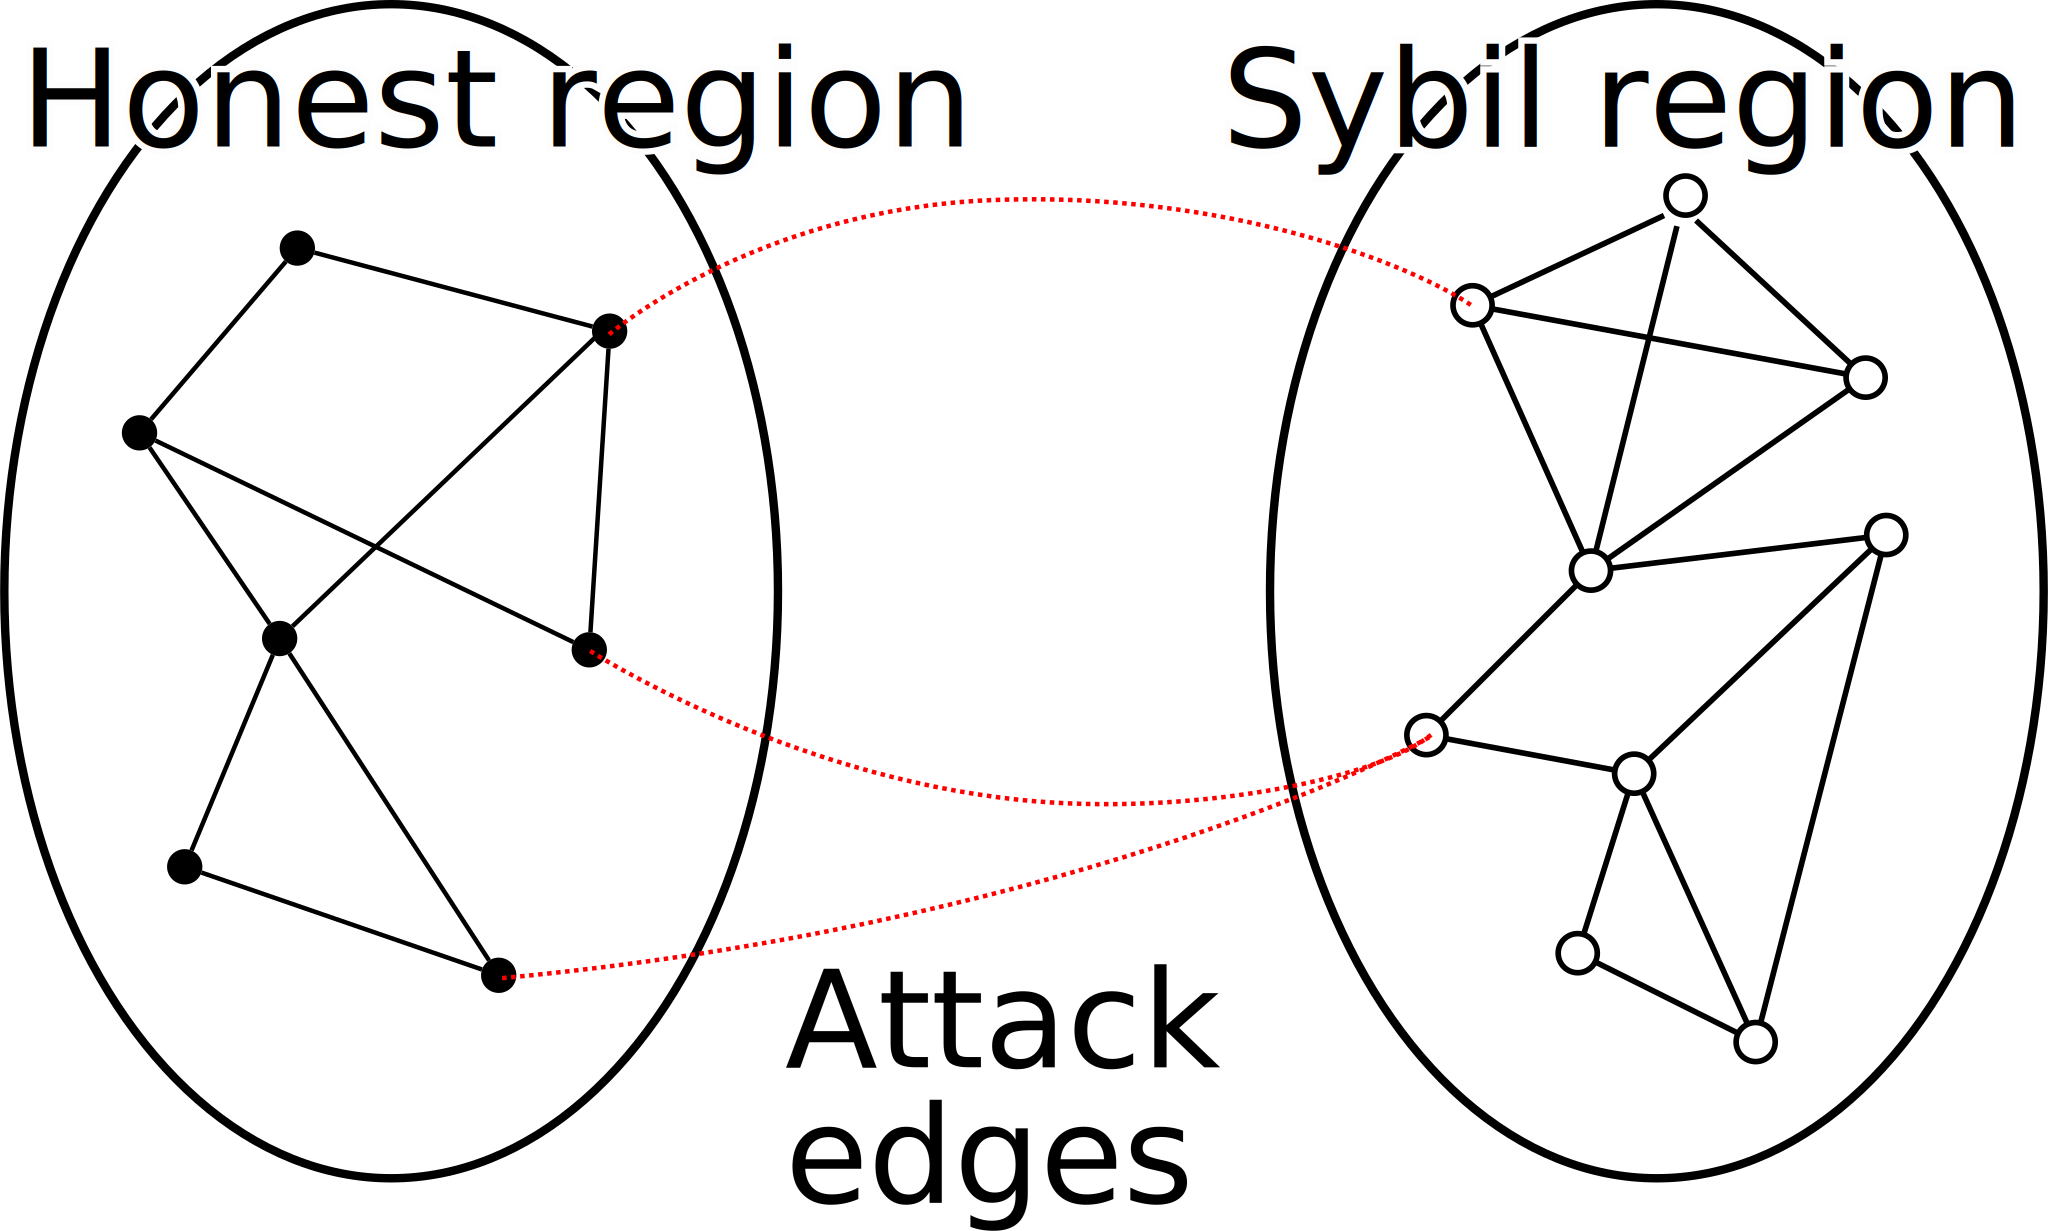
\includegraphics[width=\linewidth]{attack_edges}
  \caption{The model in many sybil defence mechanisms can be seen as a social
    graph that is partitioned into a sybil region and an honest region. The two
    regions are connected by \emph{attack edges}. Note that in general there may
    be multiple honest regions multiple sybil region. }
  \label{fig:attack-edge}
\end{figure}

A less common model is the aforementioned P2P network model \cite{douceur2002sybil}.
It does not have a notion of friendship, so sybils are free to attach themselves
with any node in the network. Only some techniques are able to defend against
sybils under this model, we describe them in \autoref{sec:network-flow}.

%%% Local Variables:
%%% mode: latex
%%% TeX-master: "main"
%%% End:


\section{Sybil Attack in Various Applications}

Sybil attacks can be mounted in different applications and cause a large array
of consequences. This section categorises the attacks by the goal for four
common applications. (1) P2P (peer-to-peer) file sharing networks such as
BitTorrent, (2) OSN (online social networks) such as Twitter and Facebook, (3)
reputation systems such as eBay and (4) WANET (wireless ad-hoc networks) such as
sensor networks. We hope this section further illuminates the alarming
consequences of the Sybil attack.

\subsection{The Sybil Attack in P2P FIle Sharing Networks}
P2P (peer-to-peer) file sharing networks are distributed computer networks that
are built for discovering and sharing files. BitTorrent\cite{bep3} is likely the
most popular P2P network at the time of writing. Due to their open and
distributed nature, they are vulnerable to the Sybil attack.

\subsubsection{Index Poisoning}
P2P networks often implement a DHT (distributed hash table). The DHT in
BitTorrent is called Mainline-DHT, based on
Kademlia\cite{maymounkov2002kademlia}. Keys are the infohashes (file
identifiers) and values are the metadata of the files, these are distributed
across all the participating peers. Every node stores a routing table and
requests are routed iteratively to the node responsible for a particular
key\cite{bep5}. The goal of index poisoning is to corrupt routing table so that
honest peers fail to find the values they want. It can be mounted by injecting
Sybils into the DHT that do not follow the protocol. Wang and Kangasharju
created honeypots in the BitTorrent network and detected as many as 300,000
Sybils\cite{wang2012real}. Similar attacks are possible in other P2P networks
such as Overnet\cite{liang2006index}.

% There are no concrete proof of malicious activities, but the Sybils can easily
% sabotage the DHT if they choose to.

% \subsubsection{Unfair Use of Resources}
% creating sybils with ``strategic'' missing pieces

% Gnutella?
% \cite{daswani2002query}
% \cite{daswani2004pong}
\subsubsection{Eclipse Attack}
Steiner et al. mounted an Eclipse attack on a Kademlia based DHT for P2P file
sharing known as KAD, it is used in Overnet and
eMule\cite{steiner2007exploiting}. The Eclipse Attack\cite{singh2006eclipse} is
a special form of targeted Sybil attack. Sybils are arranged in the network such
that they eclipse the the victim from the rest of the network. The victim can
either an identity or an object such as a key in DHT. The authors mounted the
latter variation. The authors show that it is possible to eclipse a key using
only 32 Sybils in a DHT with 1.5 million users and 42,000 key.


\subsubsection{Denial of Service}
By exploiting vulnerabilities in the BitTorrent network, denial of service
attack can be directed at any machine connected to the internet, not just
machines in the network\cite{sia2006ddos}. The main idea is to report the victim
as the tracker (a server that coordinates the peers). El Defrawy, Gjoka and
Markopoulou created a small scale proof-of-concept attack. Using only one
machine, they could generate enough traffic to cripple small organisations and
home users. The authors suggested that if Sybils are created to perform the same
attack aimed at a single victim, then it could easily throttle links with much
higher bandwidth\cite{el2007bottorrent}.

Steiner et al. also succeeded in mounting a DDoS attack but using their in the
context of the aforementioned KAD DHT\cite{steiner2007exploiting}. Instead of
replying the correct list of peers to DHT queries, the Sybils always respond
with the IP address of the target peer in an attempt to overwhelm the target.
The authors show evidence that real-world malicious DDoS attacks involving more than
300,000 peers are mounted using P2P networks.

\subsubsection{Spying}
Many authors have used Sybils to monitor or spy a P2P file sharing network that
uses DHT\cite{holz2008measurements, steiner2007exploiting}. In essence, the
authors created a lot of light-weight Sybils and trick all the honest peers to
store them in their routing table, a form of index poisoning. The Sybils are
light-weight because do not follow the DHT protocol and perform much simpler
operations, thus a single machine can have thousands of Sybils running
simultaneously. Finally, DHT requests would ``pass through'' the Sybils due to
the poisoned routing table, and the requests can be stored in a database for
further analysis. 

\subsection{The Sybil Attack in OSN}
OSN (online social networks) are vulnerable to the Sybil attack even when most
of them use a central, trusted authority such as Facebook. In OSN, users create
profiles and form relationships with friends. In contrast with real world
relationships, it is much easier to create relationships in OSN even with
strangers. In 2008, Sophos conducted an experiment where they created a Facebook
profile and send friend requests to 200 random users, and 41\% of the users
accepted the friend request\cite{sophos}. A report by Facebook at the end of
2011 stated 5-6\% of their accounts are fake\cite{facebookfake}. Combining with
the ability to create new identities with very little cost, it is possible to
perform many types of attacks which we outline below.

Note that online social networks often have a reputation aspect as well, for
example a Facebook page with a lot of fans may be considered to be more
reputable than others. We discuss attacks specific to OSN in this section and
attacks on reputation in \autoref{sec:reputation-attack}

TODO Understanding Sybil Groups\cite{jiang2015understanding}

\subsubsection{Identity Theft}
Authors of \cite{bilge2009all} created two attacks - profile cloning and
cross-site profile cloning, targeting five social network sites including
Facebook and LinkedIn. The iCloner system was created to automate these
attacks.

In profile cloning, iCloner uses publicly available information to automatically
create clones of the victim's profiles, effectively creating Sybils. iCloner
then sent friend requests from the cloned profile to the friends of the victim.
The fact that the victim may have many friends that they do not contact very
often, e.g. friend from primary school living in another country, makes this
attack highly effective. The authors found that the acceptance rate for cloned
profiles was over 60\%. Much higher than the acceptance rate of 30\% for
fictitious profiles. Once the friendship is established, it is possible to
extract private information that is not available publicly and perform identity
theft.

The idea of cross-site profile cloning is similar, except the cloned profile is
created on another social network site that the victim does not yet use. Once
the cloned profile is created, iCloner attempts to identify friends of the
victim and begins sending friend requests. Similarly, 56\% of the friend
requests were accepted. 

A more recent study created SbN (Socialbot Network) targeting
Facebook\cite{boshmaf2011socialbot}. Each socialbot is a Sybil created by the
attack, it controls a forged profile and minic human behaviour to avoid
detection. The attacker is the botmaster who coordinates the socialbots to
achieve a common objective such as infiltrating the target OSN by creating
friend relationships with real users. The authors found that infiltration
success rate was as high as 80\% and the FIS\cite{stein2011facebook} (Facebook
Immune System) was not sufficient to prevent the attack. Once the relationships
are established, the botmaster can command the socialbots to start gathering
private information which can then be used for identity theft.

% authors also said that Sybil detection based on attack edges is not effective
% because it's easy to create trust relationships with strangers

These examples demonstrate that the carelessness of users and the ability to
create Sybils makes OSN vulnerable to identity theft. Moreover, identity theft
is only an entry point. Once trust relationships are established, the attacker
can perform many other types of attacks such as spamming, phishing or
astroturfing to gain advantage.

\subsubsection{Astroturf}
Astroturfing is an act of creating grassroot movement that are in reality
carried out by a single entity, effectively spreading misinformation to
legitimate users. It relies on the ability to create Sybils in the underlying
social network. This type of attack is especially effective in social networks
such as Twitter where a lot of the social interaction such as sending messages
happen in the public.

In the 2010 Massachusetts senate race, Mustafaraj and Metaxas found evidence
that Republican campaingners created fake Twitter accounts and used them to send
spam. The spam caused Google real-time search results to tip in their favour
thus causing a spread of misinformation\cite{mustafaraj2010obscurity}.
Ratkiewicz et el. suggest that this type of attack can be mounted cheaply and
may have a larger influence than traditional
adversiting\cite{ratkiewicz2011truthy}.

The Truthy system\cite{ratkiewicz2011truthy} is a web service that perform
real-time analysis of Twitter to detect political astroturfing. In the 2010
U.S. midterm election, the authors found accounts which generated a lot of
retweets but no original tweets. More importantly, they uncovered a network of
bot accounts that injected thousands of tweets to smear the Democratic candidate.

In 2012, Wang et el. investigated two of the largeset
crowdturfing\footnote{Crowdsourced astroturfing.} platforms in China that brings
together buyers and sellers - Zhubajie and Sandaha. One of their services is
perform astroturfing on Weibo (The Chinese Twitter). The authors found that the
5364 sellers collectively own 14151 Weibo accounts and the top 1\% of the
sellers own over 100 accounts. Furthermore, the business is growing and more
than \$4 million have been spent on these two platforms over five
years\cite{wang2012serf}.

\subsubsection{Spam}
Spamming, much like in the context of email, is the act of sending unsolicited
or undesire messages (spam). The goal of the attacker varies from advertisement
to phishing and spreading malicious software\cite{twittermalware1,
  twittermalware2}. Many studies have characterised the behaviour of the
spammers and found that they either use fake accounts or stolen
accounts\cite{stringhini2010detecting, yang2012analyzing, grier2010spam}. Some
authors have worked with the service provide to close the spam accounts, but it
is clearly not sufficient as we described in \autoref{sec:motivation}.


\subsection{The Sybil Attack in Reputation Systems}\label{sec:reputation-attack}
Reputation systems cultivate collaborative behaviour by allowing entities to
trust each other based on community feedback, usually in the form of a
reputation score. Entities decide whom to trust based on the reputation scores,
thus entities are also incentivised to behave honestly. Reputation systems are
found in many context. In e-commerce, namely eBay, researchers found that the
merchant's reputation ``is a statistically and economically significant
determinant of auction prices''\cite{houser2006reputation}, and ``buyers are
willing to pay 8.1\% more'' for goods sold buy a reputable
merchant\cite{resnick2006value}. The file sharing peer-to-peer network
BitTorrent uses tit-for-tat as an ephemeral reputation system to encourage peers
to upload in exchange for better download speeds\cite{cohen2003incentives}. The
aforementioned PageRank\cite{page1999pagerank} is also a reputation system, used
for ranking reputable websites higher in Google's search results.

Unfortunately, reputation systems are also vulnerable to the Sybil attack.
Worryingly, there appears to an industry built around it, and their products are
easily accessible in the clearnet. In this section, we describe practical
attacks on reputation systems.

\subsubsection{Self-promoting}
In self-promotion, the goal of the attacker is to illegitimately raise its own
reputation. A common way to perform self-promition is to create Sybils and have
them create positive reputation for the attacker's main identity.

Dini and Spagnolo studied the economics of buying reputation on eBay. The
authors discovered many cheap items (around \euro{0.7}) for sell are simply there to
boost feedback. For example, one of the item is titled ``Apple Cranberry Crisp
Recipe + 100\% Positive Feedback''. The authors successfully boosted their
feedback by purchasing such items. But they made an unsuccessful attempted to
place a bid on their own good with a fake account\cite{dini2009buying}.

% Christin crawed the Silk Road, the anonymous marketplace. The author
% \cite{christin2013traveling}

De Cristofaro et el. performed an emperical study on Facebook page promotion
using like farms\cite{de2014paying}. Some of the farms such as
\verb!SocialFormulae.com! are clearly operated by bots and the operator does not
attempt to hide it, others such as \verb!BoostLikes.com! tries to minic human
users. The authors purchased the ``1000 likes'' service on their empty Facebook pages.
In under a month, many empty pages have accumulated almost 1000 likes as
promised by the like farms. The authors empty accounts were not terminated. Only
a small number of the liker's account were terminated.

% \cite{soska2015measuring}

SEOClerks and MyCheapJobs are also evidences of marketplaces for self-promotion.
Some of the top services include ``1 million Twitter followers'' at \$849,
``1000+ Instagram followers'' at \$10 and so on. The revenues of those two
marketplaces are estimated to be at \$1.3 million and \$116 thousand,
respectively\cite{farooqi2015characterizing}. Although the authors did not
investigate the properties of the fake followers, there is little doubt that
many of accounts used in these services are Sybils.

\subsubsection{Slandering}
The goal of a slandering attack is to illegitimately produce negative feedback
to undermine the reputation of the target. It is easy to imagine the improvement
in effectiveness when using multiple Sybils. From the best of our knowledge,
there are no published studies on real-world slandering. But
research has shown having a negative feedback may harm the target's ability to
do business\cite{ba2002evidence}.

\subsubsection{Whitewashing}
In whitewashing, attackers abuse the reputation system for temporary gain and
then escape the consequences by joining the reputation system under a new
identity to shed their bad reputation. Clearly, whitewashing is only possible
when the Sybil attack is possible. Again, there are no studies on whitewashing
in the real-world. But many have suggested that it is feasible
attack\cite{hoffman2009survey, marti2006taxonomy}.

% TODO
% \subsubsection{Denial of Service}
% The denial of service attack highly depends on the structure of the reputation
% system. 

\subsection{The Sybil Attack in WANET}
WANET (wireless ad-hoc networks) is a dynamic, self-configuring, self-healing
wireless network. Ad-hoc in this case means it does not rely on existing
infrastructure for the network to function. Each node in the network is
responsible for some general tasks such as routing, and some application
specific tasks such as gathering data from its sensors in the case of a sensor
network.

Akin to the other applications, an attacker in a WANET may own a single physical
node, but it may behave as if it were a large number of nodes. Many WANET
designs involve a reputation system\cite{ganeriwal2008reputation,
  buchegger2003robust}, thus the same attacks from
\autoref{sec:reputation-attack} applies here.
In this section we describe the WANET specific attacks. 
From the best of our knowledge WANET are not widely deployed in practice,
thus there is little research on real-world attacks.

\subsubsection{Unfair Resource Allocation}
Nodes in WANET often have limited resources such as bandwidth of the radio
channels. Resources such as these must be shared between the neighbours using
time slices. When the neighbours are Sybils, then the attacker can receive an
unfair amount of resource allocation and denies resources for the honest
nodes\cite{newsome2004sybil}. In contrast with the other attacks, this works
even when the Sybils are not behaving malicioiusly.

\subsubsection{Routing Disruption}
An important routing technique is multipath routing, data is routed using
multiple paths in the network for better fault-tolerance and bandwidth. However,
if Sybils are present in the network, then the different paths may in fact go
through the Sybils owned by the same attacker. Another technique geographic
routing, nodes route data depending on the geographic location of their
neighbours. Sybils in the network can be in more than one place at a time, thus
significant distrupting the routing algorithm\cite{karlof2003secure}.

\subsubsection{Spreading False Information}
Nodes often need to exchange information with each other to satisfy the
underlying requirements of the application. Some of the common tasks include
data aggregation, voting. With enough Sybils, it is possible to manipulate the
aggregated data or the poll to benefit the attacker. For example, sensor
networks may use a bollot to detect misbehaving nodes, the attack could use its
Sybils to claim that a honest node is misbehaving and have the other nodes expel
it from the network\cite{newsome2004sybil}.


\subsection{TODO}
a test bed for sybil attacks\cite{irissappane2012towards}

Quantifying Sybil attack\cite{margolin2008quantifying}

%%% Local Variables:
%%% mode: latex
%%% TeX-master: "main"
%%% End:


\section{Defences}\label{sec:defences}
% TODO expand, better intro
In this section we categorise various defence techniques against the
sybil-attack. Many of them are independent of the application, thus we classify
them on their main idea, and state explicitly when the mechanism is application
specific.

\subsection{Certificate Authority}\label{sec:cert-authority}

CA (certificate authorities) check the users' identities and then issues
certificates to honest users. The certificate can be tangible (trusted
hardware\cite{newsome2004sybil}) or non-tangible (public key certificate)
depending on the application. When an identity wishes to user the application,
the CA must verify the validity of its certificate to ensure one-to-one
correspondence. This mechanism prevents the Sybil attack as long as the CA does
not make mistakes in the issuance stage.

CA can prevent the Sybil attack but it also has a lot of downsides. (1) Users
have different opinions and may not agree on a single CA. (2) Users living in
authoritarian regimes may not have access to the CA in use. (3) It is difficult
to scale up a CA to meet increasing users demands. (4) Anonymity is difficult to
obtain because the CA has complete information of the entities. (5) It is a
central point of failure; i.e. if the attacker obtains the private key to create
certificates then he or she can easily generate Sybils, if the CA goes offline
then the application ceases to function because it can no longer verify
identites.

Many existing systems today use a form of CA.
X.509 is a standard for certificates and is used in a large variety of
applications, for example websites (TLS), email (S/MIME), smart cards and so on.
Payment systems such as PayPal verifies identities using credit card billing addresses.
% Credence\cite{walsh2006experience} is a distributed reputation system, but the
% identities are created using a CA.

\subsection{Resource Testing}
Every attacker can create multiple Sybils, but the attack cannot duplicate its
resources the same way. In resource testing, the goal is to find identities that
possess fewer than the expected amout of resources. The resource type can vary
depending on the application. In wireless networks it may be using radio
channels\cite{newsome2004sybil}, in online social networks it may be IP
addresses\cite{freedman2002tarzan} and solving computationally demanding puzzles
in P2P networks\cite{aspnes2005exposing}. Resource testing may deter casual
attackers but its usefulness degrades for resourceful attackers.

For example, in the Tarzan P2P network, neighbours are selected not from all
known IP addresses, but from distinct IP prefixes\cite{freedman2002tarzan}. The
effectiveness of the Sybil attack is reduced if the attackers cannot easily
create Sybils in a large range of IP prefixes.

Another example for resource
testing is self-registration\cite{dinger2006defending}. When a peer wish to join
the network, it needs to compute a ID which is a hash of its own IP address and
port number. While participating in the nettwork, other peers need to verify
that the ID matches the peer's origin.

Bitcoin is also resource testing...

SybilConf\cite{tegeler2010sybilconf}

\subsection{Registration Fee}
Using registration fee is similar to resource testing except it only happens on
registration. Entities can be charged a fee for creating identities, often 
facilitated by a central authority. The fee need to be set appropriately so that
the cost of creating Sybils outweights the benefits. The fee does not need to be
monetary. For instance, CAPTCHA\cite{von2003captcha} is a form of
registration fee. It prevents programs from automatically creating new
identities and limits the rate at which identities can be created.

TODO \cite{resnick2001social}

Feldman et el. proposed another form of registration fee for P2P networks - the
adaptive stranger policy\cite{feldman2004robust}. When new peers join the
network, they are treated using a policy that is adapted from previous
newcomers. For example, the new peers may be expected to contribute to the
network before they are allowed to receive benefits from the ``mature'' peers.
The downside is that the policy may deter honest users from joining the network
in the first place.

% Identity creation can be rate limited\cite{douceur2002sybil}, especially in the
% presence of a central authority. The limit can be set globally, or it can be
% done regionally (i.e. based on IP address).

\subsection{Network Flow Based Techniques}\label{sec:network-flow}
Network flow based techniques began with
BarterCast\cite{meulpolder2009bartercast}. It was initially designed to combat
freeriding in P2P file sharing networks, where users are selfish and do not
share content, but its idea can be extended combat the Sybil attack. The ideas
based on BarterCast do not directly identify Sybils, but they prevent Sybils
from doing harm in the P2P network.

The main idea comes from real-world social networks, where the reputation of a
person can be from direct experiences, or information obtained frome someone
else. The direct experience is always true, but the indirect information may not
be, i.e. people can lie about their experiences. Humans solve the problem by
treating the indirect information with a grain of salt unless the source of the
information is highly trusted.

BarterCast applies this idea in P2P file sharing networks. Peers all maintain a
subjective graph which is created by exchanging messages with their neighbours.
The direct experiences measured by the number of bytes uploaded and downloaded
are represented by the outgoing and incoming edges from the peer, respectively.
Indirect experiences are represented by edges that are not directly connected to
the peer. For example in \autoref{fig:bartercast}, $A$ is the subject, it has
direct experiences with $B$ and $B$ has told $A$ about $S$, so it has indirect
information about $S$. But $A$ is unsure about the truthfulness of $S$'s
contribution, so it only trusts $S$ as much as it trusts $B$. This idea is
realised using a maximum flow algorithm and the final reputation metric is given
in \autoref{eq:bartercast}.
\begin{equation}\label{eq:bartercast}
  R_i(j) = \frac{\arctan(\text{maxflow}(j, i) - \text{maxflow}(i, j))}{\pi / 2}
\end{equation}

\begin{figure}
  \centering
  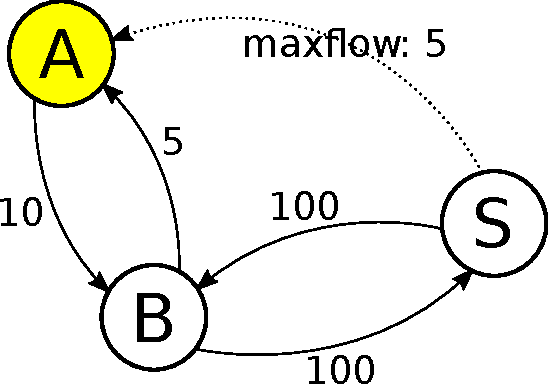
\includegraphics[width=0.3\textwidth]{bartercast}
  \caption{Subjective graph of $A$. The numbers are the amout of data transfered,
    they can be seen as the capacity in the context of the maximum flow
    problem.}
  \label{fig:bartercast}
\end{figure}

BarterCast does not prevent the Sybil attack by itself. Because attackers can
first upload a lot of data to obtain a good reputation in the network. If the
attacker now creates Sybils and false report of the Sybils saying that they
uploaded a lot. Then the peers who have interacted with the attacker will be
tricked to think that the Sybils also have a high reputation. To fix this
problem, Delaviz et el. created SybilRes\cite{delaviz2012sybilres}. The main
idea is the following. Suppose there are two peers $A$ and $B$ who are sharing
data. If $A$ is uploading (represented by an outgoing edge) to $B$, then it
decreases the weight of the incoming edge from $B$. Vice versa, the weight is
increased for the outgoing edge when $A$ is downloading. The rate of change
depends on the capacities of the edges and the amout of data transferred after
computing the reputation. Using the definition in \autoref{fig:attack-edge}, the
attacker cannot built up reputation for its Sybils by uploading to peers in the
honest region beforehand, it is now forced to keep on uploading to keep its
Sybil's reputation which is a much more desirable behaviour.

Seuken et al. provided a formal model of BarterCast. They found that BarterCast
is vulnerable to misreporting and proposed a solution called the DropEdge
mechanism\cite{seuken2011sybil, seuken2014sybil}. DropEdge, like the name
implies, drops some edges in the subjective graph that satisfies the following
constraints. Suppose peer $A$ wishes to download from peers in set $C$ (the
choice set). Then any reports received by $A$ from $p \in C$ is dropped. Also,
edges with both end points in $C$ are also dropped from $A$'s subjective graph.
Intuitively, peers in $C$ cannot misreport their contribution. The authors
formally prove this property in their work. They also prove that it is robust
against weakly benefician Sybils, that is Sybils that do not perform actual work
for honest peers.

SumUp\cite{tran2009sybil} is a defence mechanism specific for the vote
aggregation problem. For example, in social news aggregation websites such as
Reddit, users vote on the submitted content to determine its ranking; the
problem occurs when Sybils can out-vote honest users. It is a centralised
approach that fits the architecture of most websites that perform vote
aggregation. SumUp consist of three stages. Firstly, pruning is performed to
limit the number of incoming edges of every node, this is to reduce the number
of attack edges available and reduce the computational cost in later stages, the
threshold is a system parameter. Secondly, it uses a ticket source (the central
component) distributes tickets in a breadth-first search manner equally to its
neighbours, every node keeps one ticket and distributes the remaining tickets
the same way. The number of tickets distributed across an edge plus one is the
capacity of the edge. Effectively, edges closer to the ticket source have a high
capacity. This idea keeps the capacities in the Sybil region low so that they do
not have a large influence on the outcome. Finally, the maximum flow is computed
where the source is simply the ticket source and the sink is an imaginary node
with edges of capacity one that is connected to every voter. SumUp offers a
better guarantee than SybilLimit where it only accepts $1 + o(n)$ votes per
attack edge. An improved version of SumUp - GateKeeper is discussed in
\autoref{sec:random-walk}.

TODO diagram for ticket distribution?

Conversely, maximum flow is dual to minimum cut, so the problem of finding Sybil
can also be formulated as finding sparse cuts\footnote{The sparse cut problem is
  to find a partition such that the ratio between the number in the cut and the
  number of vertices in the smaller partition is minimised. This problem is
  related to minimum cut.}. Kurve and Kesidis devised an algorithm for finding
sparse cuts to detect Sybils\cite{kurve2011sybil}. Unlike the aforementioned
techniques, it relies on the presence of trusted nodes.

\subsection{Random Walk Based Techniques}\label{sec:random-walk}
TODO actually exlain SybilGuard?

Another family, possibly the largest, Sybil defence mechanism is based on random
walks. The key assumptions in these techniques is that the honest region is
\emph{fast mixing}\footnote{In a graph, if a random walk of length $O(\log{N})$
  reaches a stationary distribution of nodes, then the graph is fast mixing.},
and the attack edges are difficult to form and are independent of the number of
Sybils. The first defence mechanism is SybilGuard\cite{yu2006sybilguard},
created by Yu et el. SybilLimit\cite{yu2008sybillimit} is the continuation of
SybilGuard and it is an improvement on many fronts while keeping the same or
better guarantees as SybilGuard. In this section we focus on SybilLimit plus
other random walk based techniques.

Before explaining SybilLimit, we define the term \emph{random route}. Random
route is a modified form of a random walk. In random walk, a outgoing edge is
selected uniformly at random on every hop of the walk. In random route, every
node maintains a static routing table that contains a uniformly random
one-to-one mapping between incoming edges and outgoing edges, initialised at
start-up. Thus the route is determined by the tables on every node. An important
property of random route is that if two routes enter the same edge, then they
will always exit at the same edge, so their route after exiting will be exactly
the same. The number of hops for a random route (the mixing time) should be just
right, so that the fast mixing property is achieved only in the honest region.

In SybilLimit, every honest node acts as a verifier $V$ and initially treats all
other nodes as suspects $S$. The verification process begins by performing
multiple independent random routes by each party. $V$ labels $S$ as an honest
node if and only if they share at least one tail (the final edge in the route).
For each tail of $V$, there is a quota for the number of node that it labels.
The authors prove that SybilLimit bounds the number of accepted Sybils (false
positives) at $O(\log{n})$, an improvement from $O(\sqrt{n} \log{n})$ of
SybilGuard.

Let us consider the following three scenarios to intuitively show why SybilLimit
works. Suppose $S$ is not a Sybil, and if $V$ and $S$ perform enough random
routes, each with enough hops for fast mixing, then due to the Birthday Paradox,
$S$ and $V$ will have an intersecting tail with high probability. Next, suppose
some of the tails of $V$ are in the Sybil region so they may intersect with a
large number of Sybils, but crossing the attack edges is improbable and
accepting a lot of Sybils is also difficult due to the aforementioned quota
mechanism, thus $V$ has a small probability of accepting a large number of
Sybils. Finally, consider there is only one attack edge and suppose a Sybil has
tails in the honest region, due to the random route property, the route of the
Sybils in the honest region will be exactly the same, so accepting the Sybils in
this scenario is also low due to the quota mechanism.

TODO create a diagram for SybilLimit

SybilGuard and SybilLimit inspired many other defence mechanisms.
SybilInfer\cite{danezis2009sybilinfer} assumes trusted nodes, which create
traces by doing random walks in the graph. Based on the traces, a probability
model that descries the likelihood a trace $T$ was generated by a specific set
of honest nodes $X$, i.e. $\Pr[ T | X = \text{honest}]$. Then using Bayesian
inference, $\Pr[ X = \text{honest}| T ]$ can be computed, that is effectively
assigning a ``score'' to every node. Sybil are the nodes with a low ``score''.
SybilInfer outperforms SybilLimit regarding the number of false positives, but
its drawbacks are its high computational cost and reliance on trusted nodes.

SybilDefender\cite{wei2012sybildefender} can be seen as a two step process. It
assumes the size of the Sybil region is smaller than the honest region and the
nodes in the Sybil region are well connected. The first step is to perform
random walk to detect Sybils. The second step is to detect a complete Sybil
region around the detected Sybils. The algorithm in the second step employs
\emph{partial} random walk, where the random walk is not allowed to traverse the
same node more than once. The property of the partial random walks is that they
are likely to ``die'' (all the neighbour nodes have already been traversed) upon
reaching the edge of the Sybil region, thus they are likely to stay in the Sybil
region. The Sybil region is detected by examining the nodes traversed by the
partial random walk.

% how does SybilDefender guarantee that the Sybils actually perform the random
% walk correctly in the second step?

SybilRank, in contrast of the aforementioned techniques, is designed to be
integrated with real-world OSN and is deployed on Tuenti (an OSN with 11 million
users)\cite{cao2012aiding}. SybilRank uses short random walks that begins on
trusted nodes in the honest region. The trusted nodes is choosen manually, this
allows SybilRank to adapt to different graph structures. A novelty in SybilRank
is that it uses power iterations, an efficient technique for computing the
landing probability of random walks. Intuitively, the probability decreases for
nodes that are far away from the trusted nodes, especially for nodes in the
Sybil region. The probabilities are normalised by the degree of the node and
then ranked. The potential Sybils are the nodes that are under a some threshold.
Finally, various actions can be performed to to verify the potential Sybils,
e.g. using CAPTCHA puzzles.

SybilShield\cite{shi2013sybilshield} makes use of multiple communities. It
begins the same way as SybilGuard/SybilLimit, i.e. $V$ performs random route to
determine whether suspect $S$ is a Sybil. But to reduce the possibility that $S$
is in fact an honest node but labeled as a Sybil, $V$ searches for agents $A$
that are from another community (also using random route). $A$ performs the same
random route algorithm and decides whether $S$ is actually a Sybil and then
relay the information to $V$. If a large majority of $A$ say $S$ is honest, then
$V$ knows that it has made a mistake, otherwise $S$ is indeed a Sybil.

TODO make figure of multiple communities for SybilShield

GateKeeper\cite{tran2011optimal} combines ideas from SumUp (discussed in
\autoref{sec:network-flow}) and SybilLimit. GateKeeper assumes a admission
controller that is honest, the admission controller performs random walks to
select $n$ ticket sources. The ticket sources act the same way as SumUp where it
distributes ticket in a breadth-first search manner. For a node to be labeled
honest, it must obtain $fn$ tickets, where $f$ is a system parameter (0.2 is
shown to be a good value experimentally). This idea works becauses if the ticket
sources are evenly distributed and Sybils ony have a few attack edges, then it
is unlikely that they will receive a large number of tickets.

% Whanau\cite{lesniewski2010whanau}
% ReDS\cite{akavipat2014reds} suggests to use sybilimit or sybilinfer

\subsection{Community Detection}
Viswanath et al. realised many of the mechanisms mentioned in
\autoref{sec:random-walk} such as SybilGuard, SybilLimit and SybilInfer, are in
fact performing local community detection (i.e. detecting clusters of nodes)
which is a more developed field\cite{viswanath2010analysis}. The authors also
argue that social graphs are not always fast mixing, which may result in poor
results for techniques that uses the fast mixing assumption. Using synthetic
social graphs, the authors show that applying Mislove's
algorithm\cite{mislove2010you} achieve similar results as SybilLimit and
SybilInfer. But using a Facebook social graph, Mislove's algorithm performs
better.

SybilExposer\cite{misra2016sybilexposer}

SybilRadar\cite{mulamba2016sybilradar}

\subsection{User Feedback and Machine Learning}
In some application domains such as OSN it is possible to leverage user feedback
to detect Sybils. These techniques do not work in the general setting.

Ostra\cite{mislove2008ostra} is a system for limiting spam in social networks.
In the simplest form, every undirected edge in the social graph is considered as
two directed edges, each of them has a credit values. When a user wants to send
a message, it needs to find a path with enough credits in the social graph from
itself to the receiver. The edge traversed by the message will have its credit
deducted, and the opposite edge will have its credit added. The receiver then
decides whether the message is a spam, if it's not a spam then the credit
operations are reversed. Effectively, only spam messages will have an effect on
the credits. If a path cannot be found, i.e. all possible paths have run out of
credit, then the message is blocked. Naturally, spams from the Sybils must use
the attack edges, if enough honest users mark those messages as spam then the
credit on the attack edges will run out and the Sybils can no longer send
messages.

Stringhini et el. devised a machine learning technique to classify bot accounts 
in Twitter\cite{stringhini2010detecting}. User feedback is incoperated into the
features. For example one of features is ``FF Ratio'', that is the ratio between
number of users that the account is following and the number of followers.
Honest users typically do not follow bots and this can be considered as a form
of feedback. Other features include ``URL Ratio'', ``Message Similarity'' and so
on. The authors collected data on ``honey-profiles'', trained a classifier after
analysing those data and collaborated with Twitter to delete tens of thousands
of spam accounts.

VoteTrust\cite{xue2013votetrust} leverages the distrust relationship, i.e.
friend request rejection, to detect Sybils in OSN. Suppose $A$ sends a friend
request to $B$, if $B$ accepts/rejects the request then it is considered as a
positive/negative vote on $A$ by $B$. The first step is to use PageRank combined
with human scrutiny to select a number of trust seeds in the honest region. Then
the trusted seeds distributes \emph{vote capacity}, that is the number of votes
each node can cast. Initially only the trusted seeds have a positive vote
capacity and other nodes have 0. When a node receives a positive vote from a
trusted seed, it also receives some vote capacity. Then it can repeat the same
process on nodes it votes on, thus distributing the vote capacity. The vote
capacity decreases as it goes further away from the trusted seeds. This
technique is comparable to the ticket distribution technique used in SumUp and
GateKeeper. Finally, the votes are aggregated to compute a global ration for
every node in the graph. Naturally, the Sybils are likely to have a low vote
because their vote capacity is slow and many of their friend requests would be
rejected.

\subsection{Content Driven}
\cite{chatterjee2008robust}

\subsection{Other}
Trust transfer\cite{seigneur2005trust} is a Sybil defence mechanism for
reputation systems that transfers the reputation score from a recommender to a
recommended identity. This method discourages self-recommendation behaviour
because the attacker would need to lower the reputation of its Sybils to
recommend him or herself. The Sybils cannot gain reputation from honest
identities because if they do not interact with them. It may be strange to lose
reputation when recommending an identity, but the authors argue that in certain
scenarios where there are a lot of interactions and the overall trustworthieness
is high, then there is no major effect to transfer a little bit of reputation to
a recommended identity.

DSybil\cite{yu2009dsybil} - recommendation system, need historical data

Symon\cite{jyothi2009symon} - pair peers together, likelihood for both to be sybils is low, the pair monitor each other to prevent attacks

\subsection{Cryptography Based Techniques?}
Secure-Overlay\cite{lua2007securing} - ID crypto and SSS
Privacy-preserving\cite{schaub2016trustless} - blockchain?
Proof-of-stake\cite{dennis2016rep}

% \subsection{Unsorted?}
% 
% Beth and PGP limits Sybil attack to some extent by using social graphs
% Beth 94\cite{beth1994valuation}
% PGP (Zimmermann) 95\cite{zimmermann1995official}
% 
% Yu 00\cite{yu2000social}
% % CORE 02\cite{michiardi2002core} % MANETs
% Lee 03\cite{lee2003cooperative} - uses flooding, might not be scalable, only talks about DoS
% % Buchegger 04 - MANETs
% % Xiong 03\cite{xiong2003reputation} % also PeerTrust?
% Marti 04\cite{marti2004limited}
% ARA 05\cite{ham2005ara} - no mention of sybil, prevents freeriding, prevents short-term abuse because reputation increases gradually
% FuzzyTrust Song 05\cite{song2005trusted} - uses fuzzy logic
% P2PRep/Fuzzy 06\cite{aringhieri2006fuzzy} - also fuzzy, does not prevent generation of false rumors
% Xiong 05\cite{xiong2007countering} - no mention of sybil, but tries to mitigate false information
% PowerTrust 06\cite{zhou2007powertrust} - uses ``power nodes'' (from power-law), no mention of sybil, some defence against colluders
% % Li 07 - MANETs
% 
% Histos and Sopras\cite{zacharia2000collaborative}, doesn't really have structure?
% Beta\cite{jsang2002beta}
% % Confidant\cite{buchegger2002performance} MANETs
% Gupta et al.\cite{gupta2003reputation}
% 
% PeerTrust\cite{xiong2004peertrust} - DHT, used P-GRID source code, has credibility rating
% 
% PerContRep\cite{yan2014percontrep}


\subsection{Does not handle Sybil-attack?}
TrustMe\cite{singh2003trustme} is a reputation that focuses on anonymity, no mention of sybil attack

H-Trust\cite{zhao2009htrust} does not mention sybil

Coner et al.\cite{conner2009trust} assumes clients cannot perform sybil attack

TrustGuard 05\cite{srivatsa2005trustguard} - assumes it is built on secure overlay networks (sybil-proof networks)

Scrivener 05\cite{nandi2005scrivener} - assumes ID cannot be created and discarded

%%% Local Variables:
%%% mode: latex
%%% TeX-master: "main"
%%% End:


\section{Related Work}\label{sec:related}
Reputation Surveys:
\cite{marti2006taxonomy}
\cite{josang2007survey} ?
\cite{hoffman2009survey}
\cite{koutrouli2012taxonomy}
\cite{selvaraj2012survey} ?
\cite{hendrikx2015reputation}

Sybil Surveys:
\cite{levine2006survey}
\cite{mohaisen2013sybil}
\cite{rakesh2014survey}
\cite{gunturu2015survey}
\cite{koll2014state}
Sok\cite{alvisi2013sok} but also some contribution

Other:
\cite{wallach2003survey}

%%% Local Variables:
%%% mode: latex
%%% TeX-master: "main"
%%% End:


\section{Summary}\label{sec:summary}
In this work, we survey both the practical and the theoretical aspects of the
Sybil attack. We motivate the Sybil attack by showing the harm it is causing in
the real world. Social networks are flooded with Sybils making real news and
fake news almost indistinguishable. Users of Tor are monitored by Sybils hidden
in the network trying to reveal their real identity. Then we define the Sybil
attack using its original definition from Douceur~\cite{douceur2002sybil} and
introduce one of the most common models, i.e. the social graph. Next, we zoom
into four different systems---P2P file sharing networks, online social networks,
reputation systems and wireless ad-hoc networks---and look the various types of
attacks that can be mounted. There are a number of alarming attacks, for
instance automated identity theft, self-promotion and so on. The main part of
our work summarises the defence mechanisms. Earlier defence mechanisms primarily
work by limiting the number of identities or the rate at which they are created.
The introduction of BarterCast inspired many network-flow based techniques for
limiting the influence of Sybils. Similarly, the introduction of SybilGuard
stimulated a lot of work on random-walk based techniques for identifying Sybils.
Hybrids are also available, for instance GateKeeper is a hybrid of the two
aforementioned techniques. Finally, we compare and contrast our work with
existing surveys.

We hope this work demonstrates the alarming consequences of the Sybil attack and
many ingenious ways to defend against it. However, there does not exist a
general solution and many defence mechanisms must satisfy their own set of
assumptions in order to perform well. When the assumptions are violated, which
can be the case due to the dynamic structure of real networks, they become
ineffective (demonstrated in~\cite{liu2016smartwalk}). Moreover, almost no
defence mechanisms considers the temporal dynamics~\cite{liu2015exploiting},
i.e. the attacker may modify the attack edges or its the social graph in the
Sybil region over time. The authors show the attacker can ``greatly undermine
the security guarantees'' of many defence mechanisms.

Without a doubt, much work still needs to be done in order for the cyberspace to
be free of the Sybil attack. We hope this work serves as a cornerstone for the
future defence mechanisms.

%%% Local Variables:
%%% mode: latex
%%% TeX-master: "main"
%%% End:


\bibliographystyle{abbrv}
\bibliography{ref}

\end{document}
